\subsection{Address based stride prefetcher}
\label{sec:stridePrefetcher}
The address based stride prefetcher (ABSP) is a simplified version of the Stride Directory Prefetcher. The ABSP is based on the fact that memory accesses
often follow a stride-n pattern (where n is the number of addresses between
the accessed addressess). When accessing the members of an
array, or iterating through a loop, most of the memory accesses will
follow a stride-n pattern. An example can be shown in figure~\ref{fig:stride}.

\begin{figure}[H]
\label{fig:stride}
\centerline{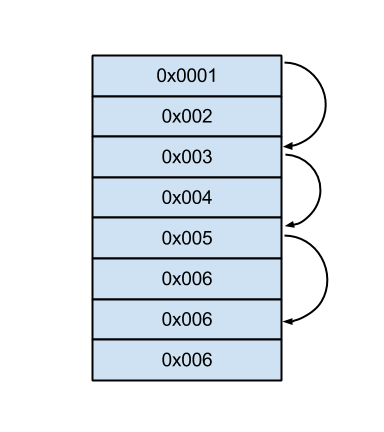
\includegraphics[scale=0.5]{./figures/stride}}
\caption{A memory access pattern with a stride of n=2}
\end{figure}

The ABSP keeps track of the last accessed address, what the delta of the addresses in the current stride is, and
also keeps track of for how long the current stride has been
ongoing. Compared to the Stride Directory Prefetcher, ABSP only requires a costant amount of memory (only the last accessed address is saved). The fact that the ABSP is an strictly \emph{address based} prefetcher also means that the \emph{realization} would be simplified since it does not need to know the value of the Program Counter.

For each memory access, the memory address is compared to the last
memory address. If the current stride value corresponds to the
difference, the number of current strides is updated. If the number of
current strides is greater than or equal to the required/configured
amunt of strides, a prefetched address is returned.  

The prefetchers can be configured by changing two variables;
the amount of strides that needs to be discovered before
the prefetcher will react on a memory access, and how many addresses it should prefetch once it is decided that it should prefetch.

